\documentclass[11pt,openany]{report}
\usepackage[spanish,es-nodecimaldot,es-tabla]{babel}
\usepackage[utf8]{inputenc}
\usepackage[T1]{fontenc}
\usepackage{lmodern}
\usepackage[a4paper,margin=2.5cm]{geometry}
\usepackage{amsmath,amssymb,amsthm,mathtools,bm}
\usepackage{graphicx}
\usepackage{booktabs,tabularx}
\usepackage{xcolor}
\usepackage[hidelinks]{hyperref}
\usepackage[style=apa,backend=biber]{biblatex}
\addbibresource{referencias.bib}

\graphicspath{{figuras/}}
% Mientras el notebook no haya generado una figura, se muestra un recuadro en su lugar.
\let\includegraphicsoriginal\includegraphics
\renewcommand{\includegraphics}[2][]{%
  \IfFileExists{figuras/#2.pdf}{\includegraphicsoriginal[#1]{#2}}{%
    \fbox{\parbox[c][4cm][c]{0.8\linewidth}{\centering Figura pendiente:\\ \texttt{\detokenize{#2}}}}}}

\theoremstyle{plain}
\newtheorem{teorema}{Teorema}[chapter]
\newtheorem{proposicion}[teorema]{Proposición}
\newtheorem{lema}[teorema]{Lema}
\theoremstyle{definition}
\newtheorem{definicion}[teorema]{Definición}
\newtheorem{hipotesis}{Hipótesis}
\renewcommand{\thehipotesis}{H\arabic{hipotesis}}
\renewcommand{\qedsymbol}{$\blacksquare$}
\renewcommand{\proofname}{Demostración}

\newcommand{\R}{\mathbb{R}}
\newcommand{\E}{\mathbb{E}}
\newcommand{\simplex}{\Delta^{N-1}}
\newcommand{\TPR}{\mathrm{TPR}}
\newcommand{\FPR}{\mathrm{FPR}}
\newcommand{\pendiente}[1]{\textcolor{orange}{[\textbf{Pendiente:} #1]}}


\title{Detección de crisis epilépticas en EEG de superficie\\[0.4em]
\large Análisis espectral, comparación de optimizadores y funciones de activación}
\author{Autor: \pendiente{nombre}\\[0.3em]Maestría en Inteligencia Artificial --- Machine Learning\\Universidad de Palermo}
\date{Diciembre de 2026}

\begin{document}
\maketitle

\begin{abstract}
\pendiente{escribir al final (unas 250 palabras): problema, datos, método, resultados principales con números, conclusión.}
\end{abstract}

\tableofcontents
\listoffigures
\listoftables

\chapter{Introducción}
\label{cap:introduccion}

\section{Motivación}

La epilepsia es una de las enfermedades neurológicas crónicas más frecuentes: afecta a unos 50 millones de personas en el mundo. Se define por la predisposición duradera a generar crisis epilépticas, episodios transitorios causados por una actividad neuronal anormalmente excesiva o sincrónica \parencite{fisher2014}. El electroencefalograma (EEG) de superficie es la herramienta central para el diagnóstico y el seguimiento, pero su revisión es manual y lenta: un registro continuo de 24 horas puede requerir horas de lectura de un especialista.

Un detector automático de crisis tiene que cumplir dos objetivos en conflicto. Debe ser \emph{sensible}, porque una crisis no detectada puede tener consecuencias graves, y \emph{específico}, porque un sistema con muchas falsas alarmas termina siendo ignorado. En la práctica clínica la especificidad suele expresarse como la cantidad de \emph{falsas alarmas por hora}.

\pendiente{ampliar a 2--3 páginas: impacto clínico, monitoreo prolongado, dispositivos portátiles, por qué el aprendizaje automático.}

\section{Planteamiento del problema}

Se aborda la detección de crisis como un problema de clasificación binaria de ventanas de EEG de 4 segundos. El problema tiene tres dificultades: (i) un fuerte desbalance de clases, porque las crisis ocupan menos del 1~\% del tiempo registrado; (ii) una gran variabilidad entre pacientes, porque la forma de una crisis cambia de una persona a otra; y (iii) la necesidad de \emph{generalizar a pacientes nuevos}, lo que obliga a evaluar con pacientes que el modelo no vio durante el entrenamiento.

\section{Objetivos}

\paragraph{Objetivo general.} Construir y evaluar un detector de crisis epilépticas basado en características espectrales del EEG y redes neuronales, y estudiar de forma controlada cómo influyen el optimizador y la función de activación en el entrenamiento y en el rendimiento.

\paragraph{Objetivos específicos.}
\begin{enumerate}
  \item Modelar matemáticamente la señal EEG y fundamentar, con la transformada de Fourier, las características espectrales que distinguen una crisis.
  \item Demostrar que la entropía espectral alcanza su máximo global en la distribución uniforme del simplex y verificar empíricamente que disminuye durante las crisis.
  \item Comparar seis optimizadores en un problema convexo y en uno no convexo, incluyendo el método del simplex de Nelder-Mead como referencia sin derivadas.
  \item Comparar cinco funciones de activación y su interacción con el optimizador y con la profundidad de la red.
  \item Evaluar el detector con curva ROC, AUC, matriz de confusión, sensibilidad y especificidad, eligiendo el umbral como un problema de optimización con restricciones.
  \item Controlar el sobreajuste con partición por paciente, regularización y \emph{early stopping}.
\end{enumerate}

\section{Hipótesis}
\label{sec:hipotesis}

\begin{hipotesis}\label{h:convexo}
En la regresión logística regularizada, que es un problema estrictamente convexo, todos los optimizadores convergen al mismo óptimo global y solo difieren en la velocidad.
\end{hipotesis}
\begin{hipotesis}\label{h:noconvexo}
En el perceptrón multicapa, que es un problema no convexo, la variabilidad del resultado entre inicializaciones es significativamente mayor que en el caso convexo.
\end{hipotesis}
\begin{hipotesis}\label{h:profundidad}
Al aumentar la profundidad, las redes con activaciones saturantes (sigmoide y tanh) se degradan más que las de la familia ReLU y GELU, por desvanecimiento del gradiente.
\end{hipotesis}
\begin{hipotesis}\label{h:adaptativos}
Los optimizadores adaptativos (RMSProp, Adam) son menos sensibles a la elección de la función de activación que SGD.
\end{hipotesis}
\begin{hipotesis}\label{h:entropia}
La entropía espectral del EEG es significativamente menor durante las crisis que fuera de ellas.
\end{hipotesis}

\section{Organización del trabajo}

El capítulo~\ref{cap:senal} presenta la fisiología del EEG y un modelo matemático de la señal. El capítulo~\ref{cap:fourier} desarrolla el análisis de Fourier y las características espectrales, incluida la entropía espectral en el simplex. El capítulo~\ref{cap:aprendizaje} formaliza el problema de aprendizaje y el sobreajuste. Los capítulos~\ref{cap:modelos} y~\ref{cap:optimizacion} tratan los modelos, las funciones de activación y los métodos de optimización. El capítulo~\ref{cap:evaluacion} define las métricas y la elección del umbral. El capítulo~\ref{cap:metodologia} describe el diseño experimental, el capítulo~\ref{cap:resultados} presenta los resultados y el capítulo~\ref{cap:conclusiones} los discute.

Todo el código está en el notebook \texttt{TP\_Final\_Crisis\_EEG.ipynb} y en los módulos de la carpeta \texttt{src/}, y puede ejecutarse localmente o en Google Colab.

\chapter{La señal EEG y su modelo matemático}
\label{cap:senal}

\section{Origen fisiológico del EEG}

El EEG de superficie registra diferencias de potencial eléctrico entre electrodos ubicados sobre el cuero cabelludo. La señal se origina principalmente en las corrientes postsinápticas de las neuronas piramidales de la corteza, que están orientadas en paralelo: cuando grandes poblaciones se activan en sincronía, sus campos se suman y generan potenciales del orden de decenas de microvoltios.

\pendiente{1--2 páginas: sistema 10-20, montaje bipolar ``doble banana'', artefactos (parpadeo, músculo, red eléctrica).}

\section{Ritmos cerebrales}

Tradicionalmente la actividad del EEG se describe en bandas de frecuencia (tabla~\ref{tab:bandas}).

\begin{table}[ht]
\centering
\caption{Bandas clásicas del EEG usadas en este trabajo.}
\label{tab:bandas}
\begin{tabular}{@{}llp{7cm}@{}}
\toprule
Banda & Rango [Hz] & Asociación típica \\
\midrule
$\delta$ (delta) & 0,5--4 & Sueño profundo; actividad lenta patológica \\
$\theta$ (theta) & 4--8 & Somnolencia; frecuente en el inicio de crisis \\
$\alpha$ (alfa) & 8--13 & Vigilia relajada con ojos cerrados \\
$\beta$ (beta) & 13--30 & Actividad cognitiva, vigilia activa \\
$\gamma$ (gamma) & 30--45 & Procesamiento local; también artefacto muscular \\
\bottomrule
\end{tabular}
\end{table}

\section{Modelo matemático de la señal}

Se modela el EEG de un canal como una suma de oscilaciones en las bandas de la tabla~\ref{tab:bandas} más un fondo aperiódico:
\begin{equation}
x(t) = \sum_{b \in \{\delta,\theta,\alpha,\beta,\gamma\}} A_b(t)\,\sin\!\big(2\pi f_b(t)\,t + \varphi_b(t)\big) + \eta(t),
\qquad S_\eta(f) \propto \frac{1}{f^{\beta}},
\label{eq:modelo_eeg}
\end{equation}
donde $A_b(t)$ y $f_b(t)$ varían lentamente respecto del período de cada oscilación y $\eta(t)$ es un proceso aleatorio cuya densidad espectral decae como una ley de potencia (ruido ``$1/f$''), con $\beta$ típicamente entre 1 y 2.

En reposo la potencia se reparte entre varias bandas y el fondo $1/f$ tiene un peso importante. Durante una crisis, una población grande de neuronas se \emph{hipersincroniza}. En el modelo~\eqref{eq:modelo_eeg} esto se traduce en:
\begin{enumerate}
  \item un término dominante $A_{b^\star}(t) \gg A_b(t)$ para $b \neq b^\star$, con $f_{b^\star}$ típicamente entre 3 y 8~Hz y a menudo con armónicos;
  \item la aparición del mismo ritmo, con fases relacionadas, en varios canales (aumento de la \emph{coherencia});
  \item un aumento de la amplitud total y de la variación de la señal en el tiempo (\emph{line length}).
\end{enumerate}

La consecuencia espectral central es que la potencia se \emph{concentra} en pocas frecuencias. El capítulo~\ref{cap:fourier} cuantifica esta concentración con la entropía espectral y demuestra que su valor máximo corresponde a una señal sin estructura (ruido blanco).

\section{La base de datos CHB-MIT}

\pendiente{describir sujetos, edades, registros, anotaciones; incluir figura \texttt{datos\_crisis} y \texttt{eeg\_crisis\_multicanal} del notebook (sección 1 y 2).}

\begin{figure}[ht]
\centering
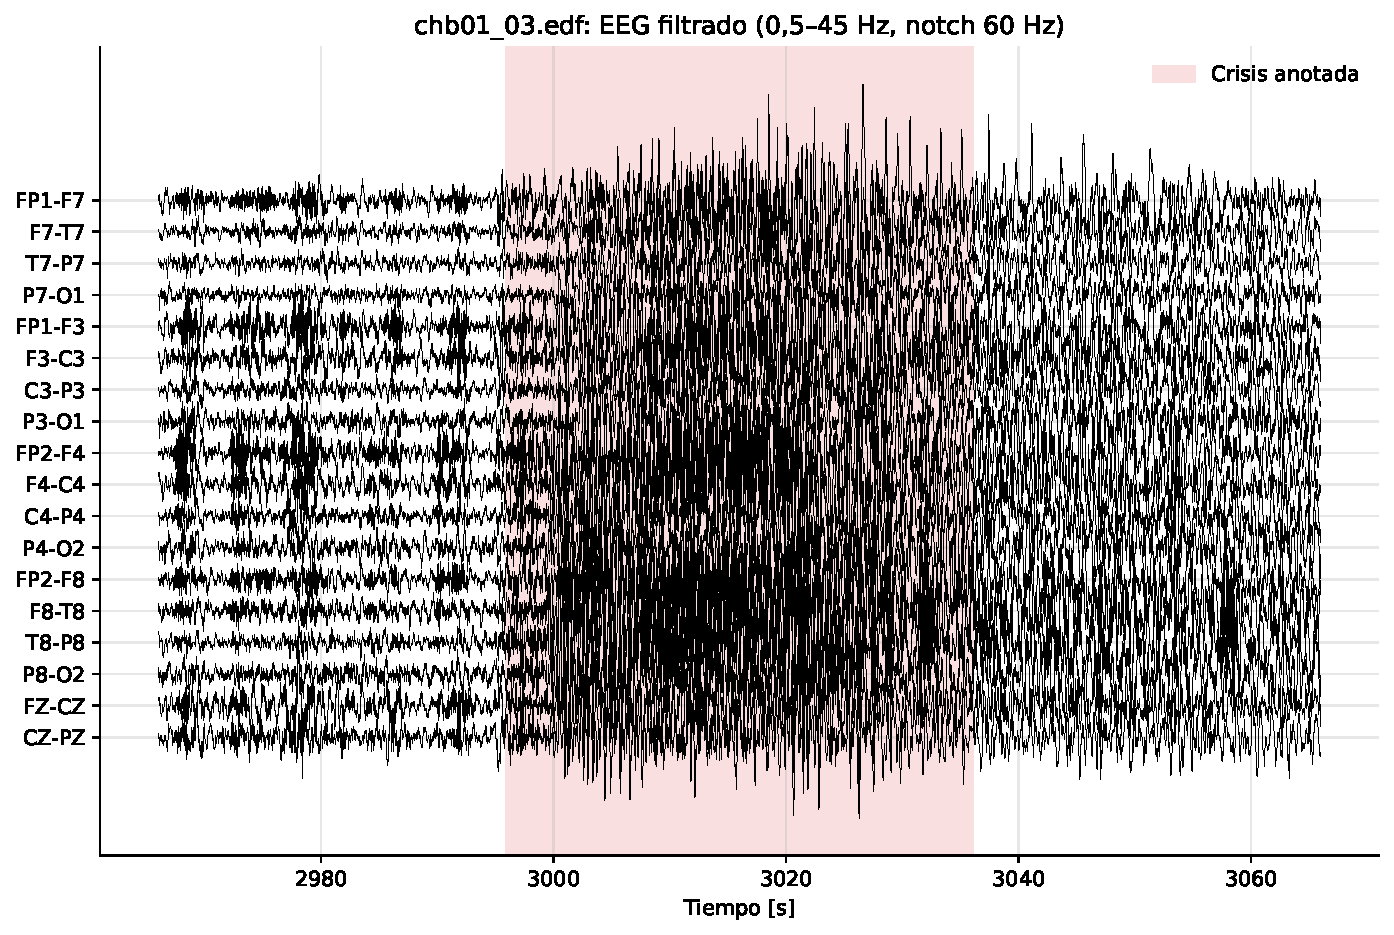
\includegraphics[width=\linewidth]{eeg_crisis_multicanal}
\caption{EEG filtrado de los 18 canales bipolares alrededor de una crisis anotada (sombreado).}
\label{fig:eeg_crisis}
\end{figure}

\chapter{Análisis de Fourier y características espectrales}
\label{cap:fourier}

\section{Serie y transformada de Fourier}

Una señal periódica de período $T$ y energía finita en un período admite la representación
\begin{equation}
x(t) = \sum_{k=-\infty}^{\infty} c_k\, e^{i 2\pi k t / T},\qquad c_k = \frac1T\int_0^T x(t)\,e^{-i2\pi k t/T}\,dt.
\end{equation}
Para señales no periódicas de energía finita se define la transformada de Fourier
\begin{equation}
X(f) = \int_{-\infty}^{\infty} x(t)\, e^{-i 2\pi f t}\, dt, \qquad x(t) = \int_{-\infty}^{\infty} X(f)\, e^{i 2\pi f t}\, df.
\end{equation}

\pendiente{propiedades: linealidad, desplazamiento, convolución $\leftrightarrow$ producto (base del filtrado); referencia a \cite{gonzalez2018}, cap.~4, y \cite{oppenheim2010}.}

\section{Muestreo y transformada discreta}

\paragraph{Teorema de muestreo (Nyquist--Shannon).} Si $X(f) = 0$ para $|f| > f_{\max}$, la señal queda completamente determinada por sus muestras $x[n] = x(n/f_s)$ siempre que $f_s > 2 f_{\max}$. Con $f_s = 256$~Hz la frecuencia de Nyquist es 128~Hz, muy por encima de los 45~Hz que se analizan.

\paragraph{Transformada discreta de Fourier (DFT).} Para $x[n]$, $n=0,\dots,N-1$:
\begin{equation}
X[k] = \sum_{n=0}^{N-1} x[n]\, e^{-i 2\pi k n/N}, \qquad f_k = \frac{k f_s}{N},\quad k = 0,\dots,N-1.
\label{eq:dft}
\end{equation}
La FFT la calcula en $O(N\log N)$ operaciones en lugar de $O(N^2)$.

\begin{teorema}[Parseval, versión discreta]\label{teo:parseval}
\[
\sum_{n=0}^{N-1} |x[n]|^2 = \frac1N \sum_{k=0}^{N-1} |X[k]|^2.
\]
\end{teorema}
\begin{proof}
Sea $\omega = e^{-i2\pi/N}$. Entonces
\[
\sum_k |X[k]|^2 = \sum_k \sum_n \sum_m x[n]\,\overline{x[m]}\,\omega^{k(n-m)}
= \sum_n \sum_m x[n]\,\overline{x[m]} \sum_k \omega^{k(n-m)}.
\]
La suma geométrica $\sum_{k=0}^{N-1}\omega^{k(n-m)}$ vale $N$ si $n=m$ y $0$ en otro caso (porque $\omega^{N(n-m)}=1$ y $\omega^{n-m}\neq 1$). Queda $\sum_k|X[k]|^2 = N\sum_n |x[n]|^2$.
\end{proof}

El teorema justifica interpretar $|X[k]|^2$ como la distribución de la energía de la señal entre las frecuencias $f_k$. En el notebook (sección~3) se verifica numéricamente sobre una ventana de EEG, con una diferencia relativa del orden de $10^{-16}$.

\section{Estimación de la densidad espectral de potencia}

\subsection{Periodograma y fuga espectral}

Cortar la señal a una ventana finita equivale a multiplicarla por una función rectangular; en frecuencia, eso es convolucionar con un núcleo de tipo $\operatorname{sinc}$ cuyos lóbulos laterales ``derraman'' potencia hacia frecuencias vecinas (\emph{fuga espectral}). Usar una ventana de Hann, $w[n] = \tfrac12\big(1 - \cos\tfrac{2\pi n}{N}\big)$, reduce fuertemente los lóbulos laterales a cambio de ensanchar el lóbulo principal.

\subsection{Método de Welch}

El periodograma de una sola ventana es un estimador \emph{inconsistente}: su varianza no disminuye al aumentar $N$. \textcite{welch1967} propuso dividir la señal en $K$ segmentos solapados de longitud $L$, ventanear cada uno y promediar:
\begin{equation}
\hat P(f_k) = \frac{1}{K}\sum_{j=1}^{K} \frac{1}{f_s \sum_n w[n]^2}\Big|\sum_{n=0}^{L-1} w[n]\, x_j[n]\, e^{-i2\pi kn/L}\Big|^2.
\label{eq:welch}
\end{equation}
Si los segmentos fueran independientes, la varianza se reduciría en un factor $K$. En este trabajo cada ventana de 4~s se divide en segmentos de 1~s con 50~\% de solapamiento ($K=7$), lo que da una resolución de 1~Hz.

\pendiente{figura \texttt{fourier\_normal\_vs\_crisis} y su discusión.}

\begin{figure}[ht]
\centering
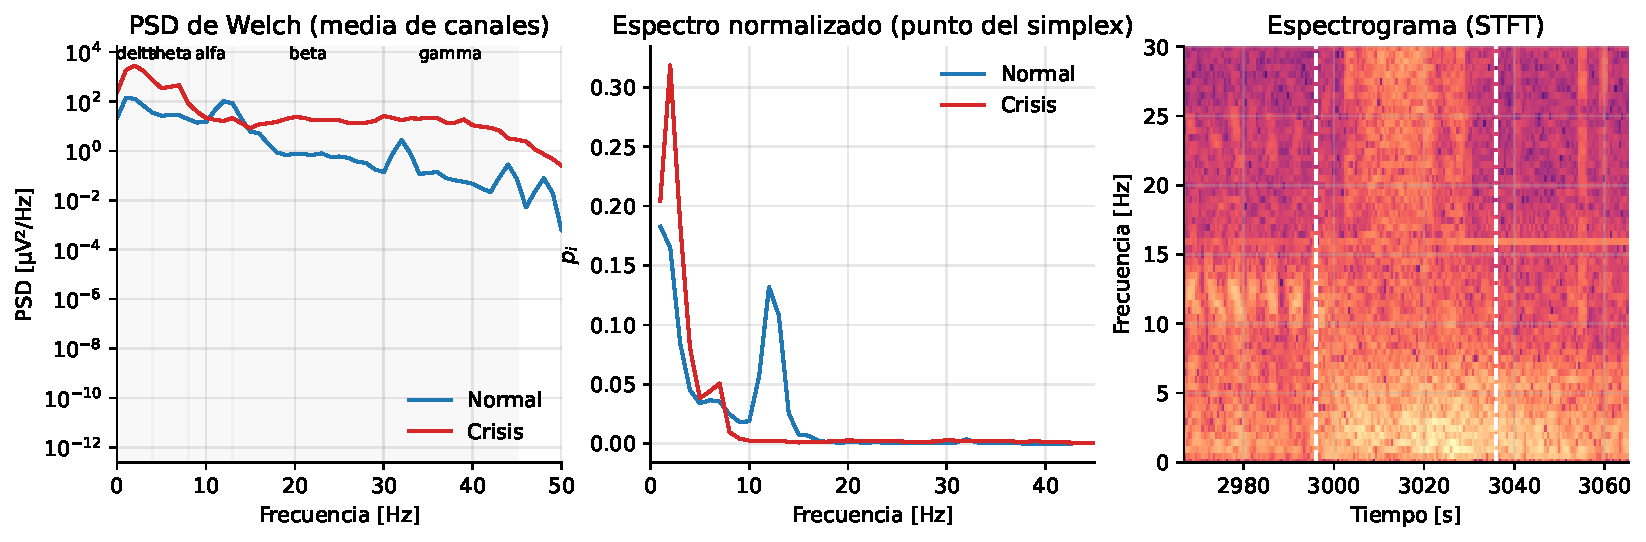
\includegraphics[width=\linewidth]{fourier_normal_vs_crisis}
\caption{Izquierda: PSD de Welch de una ventana normal y una de crisis. Centro: el mismo espectro normalizado, que es un punto del simplex. Derecha: espectrograma alrededor de la crisis.}
\label{fig:fourier}
\end{figure}

\section{Características espectrales}

Para cada canal y cada ventana se calculan:
\begin{itemize}
  \item \textbf{Potencia por banda:} $P_b = \sum_{f_k \in b} \hat P(f_k)$, en escala logarítmica.
  \item \textbf{Potencia relativa:} $r_b = P_b / \sum_{b'} P_{b'}$.
  \item \textbf{Entropía espectral} (sección~\ref{sec:entropia}).
  \item \textbf{Frecuencia dominante} $\arg\max_k \hat P(f_k)$ y \textbf{frecuencia de borde espectral} al 90~\%.
  \item \textbf{Line length} $\frac1N\sum_n |x[n+1]-x[n]|$ y log-varianza, como referencia en el dominio del tiempo.
\end{itemize}

\subsection{Coherencia entre canales}

La coherencia de magnitud cuadrada entre los canales $a$ y $b$ es
\begin{equation}
C_{ab}(f) = \frac{|S_{ab}(f)|^2}{S_{aa}(f)\,S_{bb}(f)} \in [0,1],
\end{equation}
donde $S_{ab}$ es la densidad espectral cruzada estimada también con Welch. Por la desigualdad de Cauchy--Schwarz, $|S_{ab}|^2 \le S_{aa}S_{bb}$, y vale 1 si y solo si los dos canales están relacionados por un sistema lineal. Es la medida espectral natural de la sincronización que caracteriza a una crisis.

\section{Entropía espectral, el simplex y multiplicadores de Lagrange}
\label{sec:entropia}

Al normalizar la PSD en las $N$ frecuencias de interés, $p_i = \hat P(f_i)/\sum_j \hat P(f_j)$, se obtiene un vector del \emph{simplex de probabilidad}
\begin{equation}
\simplex = \Big\{ p\in\R^N : p_i \ge 0,\ \sum_{i=1}^N p_i = 1\Big\}.
\end{equation}
El simplex es convexo y compacto: es la envolvente convexa de los $N$ vectores canónicos $e_1,\dots,e_N$. Un vértice $e_i$ representa una señal con toda su potencia en una sola frecuencia, y el baricentro $(1/N,\dots,1/N)$ representa ruido blanco.

\begin{definicion}
La \emph{entropía espectral} es $H(p) = -\sum_{i=1}^N p_i \log p_i$ (con $0\log 0 = 0$) \parencite{inouye1991}.
\end{definicion}

\begin{proposicion}\label{prop:max_entropia}
$\max_{p\in\simplex} H(p) = \log N$, y el máximo se alcanza únicamente en $p^\star = (1/N,\dots,1/N)$.
\end{proposicion}
\begin{proof}
\emph{Punto crítico.} Se plantea el lagrangiano con la restricción de igualdad:
\[
\mathcal{L}(p,\lambda) = -\sum_i p_i\log p_i + \lambda\Big(\sum_i p_i - 1\Big).
\]
La condición de primer orden $\partial\mathcal{L}/\partial p_i = -\log p_i - 1 + \lambda = 0$ da $p_i = e^{\lambda-1}$, el mismo valor para todo $i$. Con la restricción $\sum_i p_i = 1$ resulta $p_i = 1/N$ y $\lambda^\star = 1 - \log N$. En ese punto $H(p^\star) = \log N$.

\emph{Restricciones de desigualdad.} En $p^\star$ todas las componentes son positivas, así que las restricciones $p_i\ge 0$ no están activas y sus multiplicadores de KKT son nulos. Además, $\partial H/\partial p_i \to +\infty$ cuando $p_i \to 0^+$, de modo que ningún máximo puede estar en el borde del simplex.

\emph{Globalidad y unicidad.} El Hessiano es $\nabla^2 H(p) = -\operatorname{diag}(1/p_1,\dots,1/p_N) \prec 0$ en el interior del simplex: $H$ es estrictamente cóncava sobre un conjunto convexo. En un problema de maximización cóncava todo máximo local es global, y la concavidad estricta garantiza que es único.
\end{proof}

Se usa la entropía normalizada $\tilde H = H/\log N\in[0,1]$. Por la proposición~\ref{prop:max_entropia}, $\tilde H = 1$ corresponde a una potencia repartida uniformemente y $\tilde H \to 0$ a una potencia concentrada en una sola frecuencia. Según el modelo del capítulo~\ref{cap:senal}, una crisis desplaza $p$ hacia un vértice del simplex, lo que motiva la hipótesis~\ref{h:entropia}.

En el notebook (sección~4) se resuelve numéricamente el problema con un método de región de confianza con restricciones, desde varios puntos iniciales: siempre converge a $p^\star$ y al multiplicador $\lambda^\star = 1-\log N$.

\begin{figure}[ht]
\centering
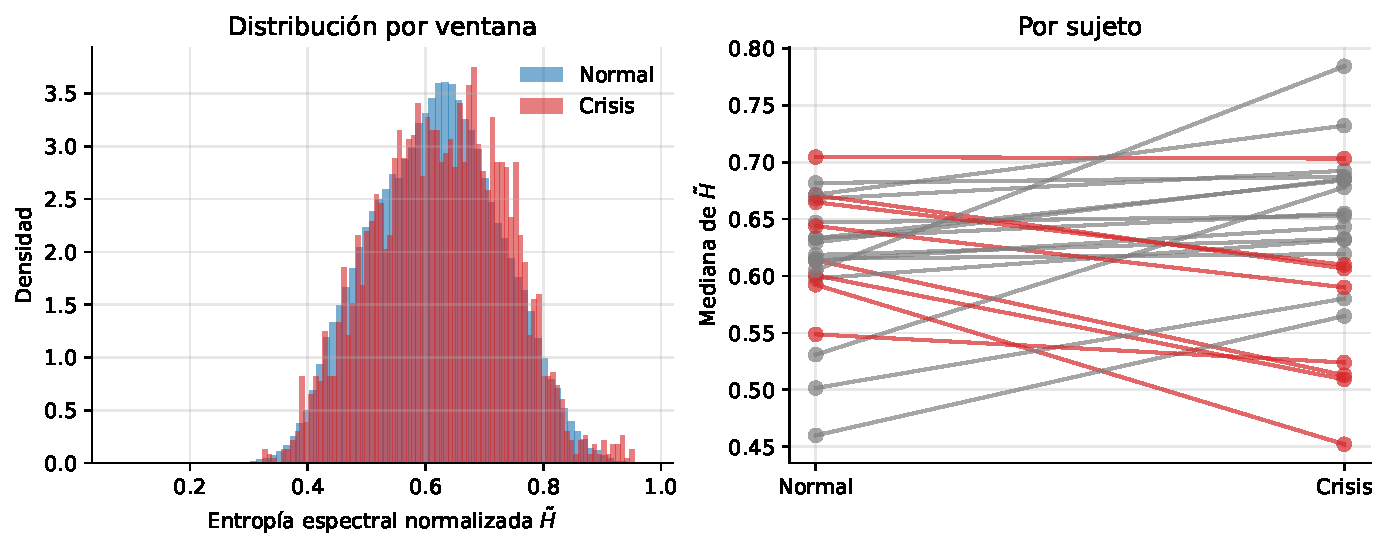
\includegraphics[width=\linewidth]{h5_entropia}
\caption{Entropía espectral normalizada en ventanas normales y de crisis (izquierda) y mediana por sujeto (derecha).}
\label{fig:h5}
\end{figure}

\pendiente{resultados numéricos de H5 (salida de la sección 5 del notebook).}

\chapter{Aprendizaje estadístico y sobreajuste}
\label{cap:aprendizaje}

\section{Formulación del problema}

Sea $(\bm x, y)$ un par aleatorio con distribución desconocida $\mathcal{D}$, donde $\bm x\in\R^d$ son las características espectrales de una ventana e $y\in\{0,1\}$ indica si hay crisis. Se busca una función $h_\theta:\R^d\to[0,1]$ que minimice el \emph{riesgo}
\begin{equation}
R(\theta) = \E_{(\bm x,y)\sim\mathcal D}\big[\ell(h_\theta(\bm x), y)\big],
\end{equation}
pero como $\mathcal D$ es desconocida se minimiza el \emph{riesgo empírico} $\hat R(\theta) = \frac1n\sum_i \ell(h_\theta(\bm x_i), y_i)$ sobre una muestra de entrenamiento.

\section{Entropía cruzada y máxima verosimilitud}

Si se modela $P(y=1\mid\bm x) = \sigma(z_\theta(\bm x))$, con $\sigma(z) = 1/(1+e^{-z})$, la log-verosimilitud negativa de la muestra es
\begin{equation}
-\log\mathcal{L}(\theta) = \sum_i \Big[-y_i\log\sigma(z_i) - (1-y_i)\log(1-\sigma(z_i))\Big] = \sum_i\Big[\log(1+e^{z_i}) - y_i z_i\Big],
\end{equation}
que es la \emph{entropía cruzada binaria} \parencite[cap.~5]{bishop2024}. Minimizarla equivale a estimar $\theta$ por máxima verosimilitud.

\subsection{Desbalance de clases}

Con una prevalencia de crisis $\pi\approx 0{,}01$, un clasificador que siempre responde ``normal'' tiene una exactitud del 99~\% y sensibilidad nula. Para compensar se pondera la pérdida: $\ell_i = c_{y_i}\,[\log(1+e^{z_i}) - y_i z_i]$ con $c_1/c_0 = (1-\pi)/\pi$. Esto equivale a entrenar como si las clases estuvieran balanceadas; el umbral de decisión se ajusta después (capítulo~\ref{cap:evaluacion}).

\pendiente{teoría de decisión bayesiana y riesgo con costos asimétricos, \cite[cap.~2]{duda2001}.}

\section{Sesgo, varianza y sobreajuste}

Para la pérdida cuadrática, el error esperado de un estimador $\hat h$ entrenado sobre una muestra aleatoria se descompone en
\begin{equation}
\E\big[(y-\hat h(\bm x))^2\big] = \underbrace{\big(\E[\hat h(\bm x)] - h^\star(\bm x)\big)^2}_{\text{sesgo}^2} + \underbrace{\operatorname{Var}\big[\hat h(\bm x)\big]}_{\text{varianza}} + \underbrace{\sigma^2}_{\text{ruido}}.
\end{equation}
Un modelo con mucha capacidad reduce el sesgo pero aumenta la varianza: se ajusta a particularidades de la muestra de entrenamiento (\emph{sobreajuste}) y generaliza mal.

\pendiente{demostración de la descomposición; figura conceptual.}

\section{Regularización}

\begin{itemize}
  \item \textbf{Penalización $L_2$:} minimizar $\hat R(\theta) + \frac\mu2\|\theta\|^2$. Por dualidad de Lagrange es equivalente a minimizar $\hat R$ sujeto a $\|\theta\|^2\le r^2$ para algún $r$ que depende de $\mu$ \parencite[sec.~7.2]{goodfellow2016}. En AdamW se aplica como decaimiento de pesos desacoplado \parencite{loshchilov2019}.
  \item \textbf{Dropout:} en cada paso se anula aleatoriamente cada unidad oculta con probabilidad $q$, lo que equivale aproximadamente a promediar un ensamble de subredes.
  \item \textbf{Early stopping:} se detiene el entrenamiento cuando el desempeño en validación deja de mejorar. Para modelos lineales con pérdida cuadrática es equivalente a una regularización $L_2$ \parencite[sec.~7.8]{goodfellow2016}.
\end{itemize}

\section{Fuga de información y partición por paciente}

Las ventanas consecutivas de un mismo registro son casi idénticas. Si se reparten al azar entre entrenamiento y prueba, el modelo puede ``reconocer al paciente'' en lugar de aprender a detectar crisis, y la métrica de prueba queda inflada. Por eso todas las ventanas de un mismo sujeto van al mismo conjunto. En CHB-MIT, además, los casos \texttt{chb01} y \texttt{chb21} son la misma paciente y se tratan como un único sujeto.

\pendiente{comparación partición por sujeto vs. aleatoria (sección 11 del notebook), figura \texttt{sobreajuste\_curvas}.}

\chapter{Modelos y funciones de activación}
\label{cap:modelos}

\section{Regresión logística}

El modelo es $P(y=1\mid\bm x) = \sigma(\bm w^\top\bm x + b)$. La frontera de decisión es el hiperplano $\bm w^\top\bm x + b = t'$ y la pérdida (capítulo~\ref{cap:aprendizaje}) es convexa en $(\bm w, b)$, como se demuestra en el capítulo~\ref{cap:optimizacion}.

\section{Máquinas de vectores soporte y dualidad de Lagrange}

\pendiente{2--3 páginas: problema primal de margen máximo, lagrangiano, condiciones KKT, problema dual, vectores soporte \cite[cap.~5]{duda2001}. Se presenta como ejemplo clásico del uso de multiplicadores de Lagrange; no forma parte de la comparación experimental.}

\section{Perceptrón multicapa}

Una red de $L$ capas ocultas calcula
\begin{equation}
\bm h^{(0)} = \bm x,\qquad \bm z^{(l)} = W^{(l)}\bm h^{(l-1)} + \bm b^{(l)},\qquad \bm h^{(l)} = \phi(\bm z^{(l)}),\qquad z = \bm w^\top \bm h^{(L)} + b,
\end{equation}
con salida $\sigma(z)$. Para clasificación en $K$ clases la salida sería $\operatorname{softmax}(\bm z)_k = e^{z_k}/\sum_j e^{z_j}$, cuyo vector de salida vive en el simplex $\Delta^{K-1}$; en el caso binario se reduce a la sigmoide.

\section{Teorema de aproximación universal}

\begin{teorema}[\cite{leshno1993}]
Sea $\phi:\R\to\R$ continua. El conjunto de funciones $\{\sum_{j=1}^m a_j\,\phi(\bm w_j^\top\bm x + b_j)\}$ es denso en $C(K)$ para todo compacto $K\subset\R^d$ si y solo si $\phi$ no es un polinomio.
\end{teorema}

El resultado generaliza el de \textcite{cybenko1989} para funciones sigmoidales y justifica que todas las activaciones comparadas sean, en principio, suficientes. Las diferencias prácticas entre ellas no están en lo que \emph{pueden} representar sino en lo fácil que es \emph{entrenarlas} con descenso por gradiente.

\section{Funciones de activación comparadas}

\begin{table}[ht]
\centering
\caption{Funciones de activación y sus derivadas.}
\label{tab:activaciones}
\renewcommand{\arraystretch}{1.4}
\begin{tabular}{@{}lll@{}}
\toprule
Activación & $\phi(z)$ & $\phi'(z)$ \\
\midrule
Sigmoide & $\sigma(z) = \dfrac{1}{1+e^{-z}}$ & $\sigma(z)(1-\sigma(z)) \le \tfrac14$ \\
Tanh & $\tanh z$ & $1-\tanh^2 z \le 1$ \\
ReLU & $\max(0,z)$ & $\mathbb{1}[z>0]$ \\
Leaky ReLU & $\max(\alpha z, z)$, $\alpha = 0{,}01$ & $1$ si $z>0$; $\alpha$ si $z<0$ \\
GELU & $z\,\Phi(z)$ & $\Phi(z) + z\,\varphi(z)$ \\
\bottomrule
\end{tabular}
\end{table}

\begin{proposicion}
$\sigma'(z) \le 1/4$, con igualdad solo en $z = 0$.
\end{proposicion}
\begin{proof}
$\sigma'(z) = s(1-s)$ con $s = \sigma(z)\in(0,1)$. La función $s(1-s)$ es una parábola cóncava con máximo $1/4$ en $s = 1/2$, es decir, en $z=0$.
\end{proof}

\pendiente{gráfico de las 5 funciones y sus derivadas; discusión de saturación, salida centrada en cero, neuronas muertas, suavidad (GELU, \cite{hendrycks2016}) y subgradiente de ReLU en 0.}

\section{Propagación del gradiente y desvanecimiento}

Por la regla de la cadena,
\begin{equation}
\frac{\partial \mathcal{L}}{\partial \bm h^{(l)}} = \Big(\prod_{k=l+1}^{L} W^{(k)\top} D^{(k)}\Big)\frac{\partial\mathcal{L}}{\partial\bm h^{(L)}},\qquad D^{(k)} = \operatorname{diag}\big(\phi'(\bm z^{(k)})\big).
\end{equation}
Tomando normas, $\big\|\partial\mathcal L/\partial\bm h^{(l)}\big\| \le \prod_{k>l}\|W^{(k)}\|\,\|D^{(k)}\|\;\big\|\partial\mathcal L/\partial\bm h^{(L)}\big\|$. Con la sigmoide $\|D^{(k)}\|\le 1/4$, así que si los pesos tienen norma cercana a 1 el gradiente que llega a la capa $l$ se atenúa al menos como $(1/4)^{L-l}$: las primeras capas casi no aprenden. Con ReLU, $\|D^{(k)}\|\le 1$ y la activación no atenúa el gradiente, pero una unidad con $z\le 0$ para todas las entradas tiene gradiente nulo para siempre (\emph{unidad muerta}). Leaky ReLU evita este problema con una pendiente $\alpha>0$ para $z<0$ \parencite{maas2013}.

\section{Inicialización según la activación}

Considérese $z_j = \sum_{i=1}^{n_{\text{in}}} W_{ji} h_i$ con $W_{ji}$ independientes, de media cero y varianza $v$, independientes de $h_i$. Entonces $\operatorname{Var}(z_j) = n_{\text{in}}\, v\, \E[h_i^2]$.
\begin{itemize}
  \item \textbf{Glorot/Xavier} \parencite{glorot2010}: para activaciones aproximadamente lineales cerca de 0 (tanh), conservar la varianza hacia adelante y hacia atrás lleva al compromiso $v = 2/(n_{\text{in}} + n_{\text{out}})$.
  \item \textbf{He/Kaiming} \parencite{he2015}: con ReLU y $z$ simétrica, $\E[h^2] = \tfrac12\operatorname{Var}(z)$, de modo que conservar la varianza exige $v = 2/n_{\text{in}}$.
\end{itemize}
Para que la comparación de activaciones sea justa, cada una se usa con la inicialización que le corresponde.

\pendiente{desarrollo completo de las dos derivaciones.}

\chapter{Optimización}
\label{cap:optimizacion}

\section{Optimalidad local y global}

\begin{definicion}
Sea $f:\R^d\to\R$. Un punto $\theta^\star$ es un \emph{mínimo global} si $f(\theta^\star)\le f(\theta)$ para todo $\theta$, y un \emph{mínimo local} si existe $\varepsilon>0$ tal que $f(\theta^\star)\le f(\theta)$ para todo $\theta$ con $\|\theta-\theta^\star\|<\varepsilon$.
\end{definicion}

\paragraph{Condiciones de optimalidad.} Si $f$ es dos veces diferenciable y $\theta^\star$ es un mínimo local, entonces $\nabla f(\theta^\star) = 0$ (primer orden) y $\nabla^2 f(\theta^\star)\succeq 0$ (segundo orden necesaria). Si $\nabla f(\theta^\star) = 0$ y $\nabla^2 f(\theta^\star)\succ 0$, entonces $\theta^\star$ es un mínimo local estricto (segundo orden suficiente) \parencite[cap.~2]{nocedal2006}.

\section{Convexidad}

\begin{definicion}
$f$ es convexa si $f(\alpha\theta + (1-\alpha)\theta')\le\alpha f(\theta)+(1-\alpha)f(\theta')$ para todo $\theta,\theta'$ y $\alpha\in[0,1]$, y estrictamente convexa si la desigualdad es estricta cuando $\theta\ne\theta'$ y $\alpha\in(0,1)$.
\end{definicion}

\begin{teorema}\label{teo:local_global}
Si $f$ es convexa, todo mínimo local es global. Si además es estrictamente convexa, el mínimo global (si existe) es único.
\end{teorema}
\begin{proof}
Sea $\theta^\star$ un mínimo local y supóngase que existe $\theta'$ con $f(\theta') < f(\theta^\star)$. Para $\alpha\in(0,1]$, $f(\theta^\star + \alpha(\theta'-\theta^\star)) \le (1-\alpha)f(\theta^\star) + \alpha f(\theta') < f(\theta^\star)$. Tomando $\alpha$ suficientemente chico, el punto queda dentro de cualquier entorno de $\theta^\star$, lo que contradice que sea mínimo local. Para la unicidad: si $\theta_1\ne\theta_2$ fueran dos mínimos globales con valor $f^\star$, por convexidad estricta $f(\tfrac12\theta_1+\tfrac12\theta_2)<f^\star$, absurdo.
\end{proof}

\begin{proposicion}\label{prop:logistica_convexa}
La pérdida logística regularizada
\[
f(\bm w,b) = \frac1n\sum_i c_i\big[\log(1+e^{z_i}) - y_i z_i\big] + \frac\mu2\|\bm w\|^2,\qquad z_i = \bm w^\top\bm x_i + b,\ c_i>0,
\]
es convexa en $(\bm w, b)$, y estrictamente convexa en $\bm w$ si $\mu > 0$.
\end{proposicion}
\begin{proof}
Con $\tilde{\bm x}_i = (\bm x_i, 1)$, el gradiente es $\nabla f = \frac1n\sum_i c_i(\sigma(z_i) - y_i)\tilde{\bm x}_i + \mu(\bm w,0)$ y el Hessiano
\[
\nabla^2 f = \frac1n \tilde X^\top D\tilde X + \mu\begin{pmatrix} I & 0\\ 0 & 0\end{pmatrix},\qquad D = \operatorname{diag}\big(c_i\,\sigma(z_i)(1-\sigma(z_i))\big).
\]
Como $D$ tiene diagonal positiva, $\bm v^\top\tilde X^\top D\tilde X\bm v = \sum_i D_{ii}(\tilde{\bm x}_i^\top\bm v)^2\ge 0$, y el término de regularización suma $\mu\|\bm v_{\bm w}\|^2 > 0$ para toda dirección con componente no nula en $\bm w$.
\end{proof}

En cambio, la pérdida de una red con al menos una capa oculta no es convexa: basta observar que permutar las unidades de una capa oculta da otra red con exactamente la misma salida, de modo que si $\theta^\star$ es un mínimo con unidades distintas, sus permutaciones son mínimos distintos con el mismo valor, y por el teorema~\ref{teo:local_global} una función estrictamente convexa no puede tenerlos. Por eso, en el caso no convexo, el punto de llegada depende de la inicialización y del optimizador (hipótesis~\ref{h:noconvexo}).

\section{Descenso por gradiente}

\pendiente{tasa de convergencia para $f$ $L$-suave y $\mu$-fuertemente convexa: $f(\theta_t)-f^\star\le(1-\mu/L)^t(f(\theta_0)-f^\star)$; número de condición.}

\section{Descenso por gradiente estocástico}

\pendiente{estimador insesgado del gradiente; con tasa constante, SGD converge a una vecindad de $\theta^\star$ de tamaño $O(\eta)$, lo que explica la brecha observada en la figura~\ref{fig:convexo}.}

\section{Momento y aceleración de Nesterov}

\pendiente{ecuaciones de momento clásico y de Nesterov \parencite{sutskever2013}; interpretación como bola pesada.}

\section{Métodos adaptativos: RMSProp, Adam y AdamW}

\pendiente{ecuaciones de RMSProp \parencite{tieleman2012}, Adam con corrección de sesgo \parencite{kingma2015} y AdamW \parencite{loshchilov2019}; discusión de \textcite{wilson2017}.}

\section{Métodos cuasi-Newton: L-BFGS}

\pendiente{paso de Newton, condición de secante, actualización BFGS, memoria limitada, búsqueda lineal con condiciones de Wolfe fuertes \parencite{liu1989,nocedal2006}.}

\section{El método del simplex de Nelder-Mead}

\pendiente{operaciones de reflexión, expansión, contracción y encogimiento sobre un simplex de $d+1$ vértices \parencite{nelder1965}; no usa derivadas; costo y falta de garantías de convergencia en dimensión alta.}

\begin{figure}[ht]
\centering
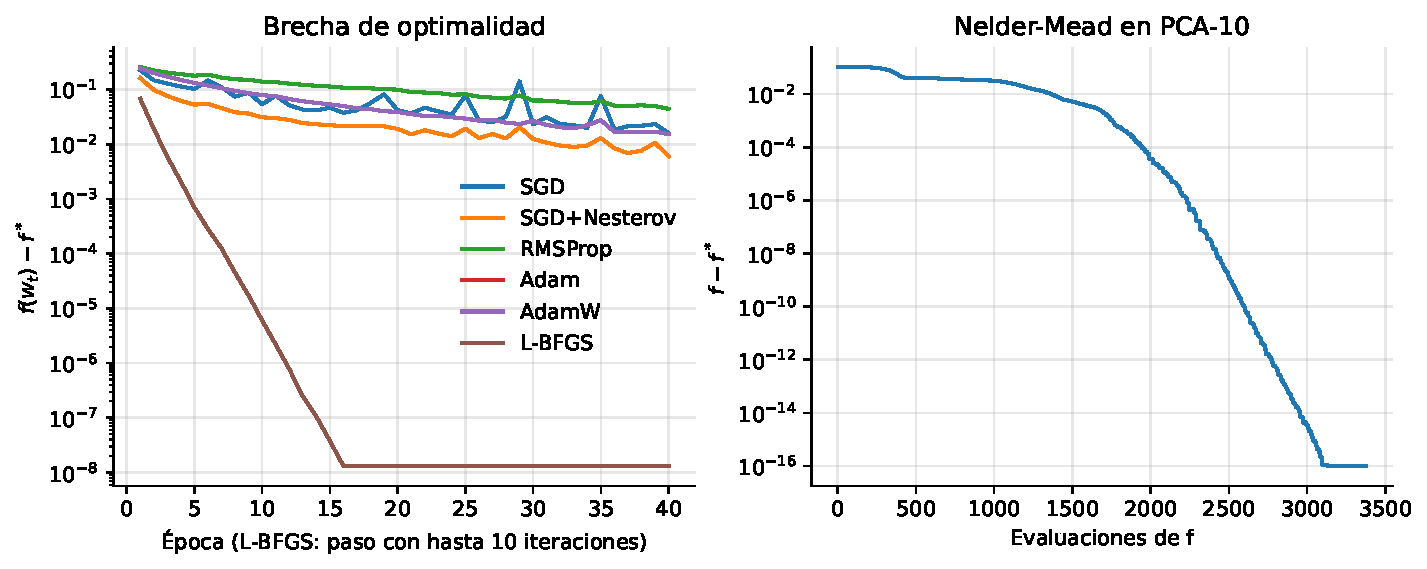
\includegraphics[width=\linewidth]{convexo_brecha}
\caption{Brecha de optimalidad $f(w_t)-f^\star$ en la regresión logística regularizada (izquierda) y de Nelder-Mead en un subespacio de 10 dimensiones (derecha).}
\label{fig:convexo}
\end{figure}

\chapter{Evaluación de clasificadores}
\label{cap:evaluacion}

\section{Matriz de confusión}

Dado un umbral $t$ sobre el puntaje $s(\bm x)$, se predice crisis si $s(\bm x)\ge t$. La matriz de confusión cuenta verdaderos positivos (VP), falsos positivos (FP), verdaderos negativos (VN) y falsos negativos (FN). A partir de ella:
\begin{align}
\text{Sensibilidad} = \TPR(t) &= \frac{VP}{VP+FN}, &
\text{Especificidad} = 1-\FPR(t) &= \frac{VN}{VN+FP},\\
\text{VPP (precisión)} &= \frac{VP}{VP+FP}, &
F_1 &= \frac{2\,\text{VPP}\cdot\text{Sens.}}{\text{VPP}+\text{Sens.}}.
\end{align}
Con ventanas de $\Delta = 4$~s, las falsas alarmas por hora son $FP / \big((VN+FP)\,\Delta/3600\big)$.

\section{Curva ROC y AUC}

La curva ROC es el conjunto de puntos $(\FPR(t), \TPR(t))$ al recorrer todos los umbrales \parencite{fawcett2006}. El área bajo la curva tiene una interpretación probabilística:
\begin{proposicion}
$\mathrm{AUC} = P\big(s(\bm x^+) > s(\bm x^-)\big)$, donde $\bm x^+$ y $\bm x^-$ son una ventana de crisis y una normal elegidas al azar e independientes (contando los empates con peso $1/2$).
\end{proposicion}
\pendiente{demostración (relación con el estadístico U de Mann-Whitney).}

Con clases muy desbalanceadas, la curva ROC puede ser engañosamente optimista porque el FPR se calcula sobre una clase enorme. Por eso también se reporta la curva precisión-recall y su área (AP) \parencite{saito2015}.

\section{Elección del umbral como problema de optimización}

\subsection{Índice de Youden}
Sin restricciones, se elige $t$ que maximiza $J(t) = \TPR(t) - \FPR(t)$, el punto de la ROC más alejado de la diagonal.

\subsection{Criterio de Neyman-Pearson y multiplicador de Lagrange}

En un detector clínico la restricción natural es un máximo de falsas alarmas. Se plantea
\begin{equation}
\max_t\ \TPR(t)\quad\text{sujeto a}\quad\FPR(t)\le\alpha,
\label{eq:np}
\end{equation}
con $\alpha = 1\cdot\Delta/3600\approx 0{,}0011$, equivalente a una falsa alarma por hora. El lagrangiano es
\begin{equation}
\mathcal{L}(t,\lambda) = \TPR(t) - \lambda\big(\FPR(t)-\alpha\big),\qquad\lambda\ge 0.
\end{equation}
Si se parametriza la curva por $u = \FPR$ y $\TPR = g(u)$ es cóncava (lo que se garantiza reemplazando la ROC por su envolvente cóncava), las condiciones KKT son:
\[
g'(u^\star) = \lambda^\star,\qquad \lambda^\star(u^\star-\alpha) = 0,\qquad u^\star\le\alpha,\qquad\lambda^\star\ge 0.
\]
Como $g$ es creciente, la restricción está activa ($u^\star = \alpha$) y \textbf{el multiplicador óptimo es la pendiente de la ROC en el punto de operación}.

\begin{teorema}[Lema de Neyman-Pearson, \cite{neyman1933}]
Entre todos los tests con $\FPR\le\alpha$, el de mayor $\TPR$ rechaza la hipótesis nula (``normal'') cuando el cociente de verosimilitudes $\Lambda(s) = p(s\mid\text{crisis})/p(s\mid\text{normal})$ supera un umbral $\eta$ elegido para que $\FPR = \alpha$.
\end{teorema}

Además, si el puntaje es monótono en $\Lambda$, la pendiente de la ROC en el umbral $t$ es exactamente $\Lambda(t) = p(t\mid 1)/p(t\mid 0)$ \parencite{fawcett2006}. Por lo tanto $\lambda^\star = \eta$: el multiplicador de Lagrange del problema~\eqref{eq:np} es el umbral del lema de Neyman-Pearson, y se interpreta como cuántas veces más probable es el puntaje bajo crisis que bajo normalidad en la frontera de decisión. También es el ``precio sombra'' de la restricción: $d\,\TPR^\star/d\alpha = \lambda^\star$ indica cuánta sensibilidad se gana por cada unidad adicional de FPR permitida.

\pendiente{demostración del lema; figura \texttt{evaluacion\_final}.}

\section{Métricas por evento}

\pendiente{sensibilidad por crisis y latencia de detección.}

\section{Pruebas estadísticas para comparar modelos}

\pendiente{Friedman, Wilcoxon de rangos con signo, corrección de Holm, ANOVA de dos factores con interacción \parencite{demsar2006}.}

\chapter{Metodología experimental}
\label{cap:metodologia}

\section{Datos y selección de registros}

Se usó la base CHB-MIT Scalp EEG Database, versión 1.0.0 \parencite{shoeb2009,goldberger2000}. Se descargaron todos los registros con crisis anotadas y tres registros sin crisis por caso, elegidos al azar con semilla fija, verificando cada archivo con su suma SHA-256. Las etiquetas se tomaron de los archivos \texttt{chbXX-summary.txt}. Se detectó una inconsistencia en los metadatos de la base: \texttt{RECORDS-WITH-SEIZURES} lista \texttt{chb07\_18.edf}, pero el resumen ubica la crisis en \texttt{chb07\_19.edf}; se usó la unión de ambas fuentes para la descarga y el resumen para las etiquetas.

\pendiente{tabla de sujetos (sección 1 del notebook): horas, crisis, duración.}

\section{Preprocesamiento}

\begin{enumerate}
  \item Selección de los 18 canales bipolares del montaje ``doble banana'' presentes en todos los registros; se descartan los archivos que no los tienen.
  \item Filtro Butterworth pasabanda de orden 4 entre 0,5 y 45~Hz y filtro \emph{notch} en 60~Hz ($Q=30$), ambos aplicados hacia adelante y hacia atrás (fase cero).
  \item Ventanas de 4~s sin solapamiento. Una ventana se etiqueta como crisis si al menos el 50~\% de su duración cae dentro de una crisis anotada.
\end{enumerate}

\section{Características}

Por canal: log-potencia y potencia relativa en 5 bandas, entropía espectral normalizada, frecuencia dominante, frecuencia de borde al 90~\%, \emph{line length} y log-varianza (15 características). Por ventana: coherencia media entre los 153 pares de canales en cada banda (5). Total: $18\times 15 + 5 = 275$ características, estandarizadas con media y desvío del conjunto de entrenamiento.

\section{Partición}

\pendiente{sujetos en entrenamiento / validación / prueba y cantidad de ventanas (sección 5 del notebook).}

\section{Modelos y entrenamiento}

\begin{itemize}
  \item Regresión logística y perceptrón multicapa de dos capas ocultas (128 y 64 unidades) con \emph{dropout} 0,2.
  \item Entropía cruzada binaria ponderada por clase, minilotes de 256, hasta 40 épocas con \emph{early stopping} (paciencia 8) sobre el AUC de validación.
  \item Para L-BFGS cada época es un paso sobre el conjunto completo con hasta 10 iteraciones y búsqueda lineal de Wolfe fuerte.
\end{itemize}

\section{Diseño de los experimentos}

\begin{table}[ht]
\centering
\caption{Experimentos realizados.}
\label{tab:experimentos}
\begin{tabularx}{\linewidth}{@{}lXl@{}}
\toprule
Experimento & Factores & Hipótesis \\
\midrule
Convexo & 6 optimizadores + Nelder-Mead sobre regresión logística $L_2$; brecha a $f^\star$ & \ref{h:convexo} \\
Ajuste de tasa & 3--4 tasas por optimizador, red ReLU, semilla 0 & --- \\
Grilla & 6 optimizadores $\times$ 5 activaciones $\times$ 5 semillas = 150 & \ref{h:noconvexo}, \ref{h:adaptativos} \\
Logística & 6 optimizadores $\times$ 5 semillas, sin capas ocultas & \ref{h:noconvexo} \\
Profundidad & 2, 4, 8 capas $\times$ 4 activaciones $\times$ 3 semillas, SGD+Nesterov & \ref{h:profundidad} \\
Entropía & ventanas normales vs. crisis, por ventana y por sujeto & \ref{h:entropia} \\
\bottomrule
\end{tabularx}
\end{table}

\section{Reproducibilidad}

Todo el código está en el notebook \texttt{TP\_Final\_Crisis\_EEG.ipynb} y en los módulos de \texttt{src/}. Las semillas están fijadas, cada entrenamiento se guarda en un archivo de resultados y los experimentos se pueden interrumpir y reanudar. El entorno usado fue Python 3.12 con PyTorch, scikit-learn, SciPy y statsmodels.

\chapter{Resultados}
\label{cap:resultados}

\pendiente{completar con las salidas del notebook ejecutado con \texttt{MODO\_RAPIDO = False}.}

\section{Entropía espectral (H5)}
\pendiente{sección 5 del notebook; figura~\ref{fig:h5}.}

\section{Caso convexo (H1)}
\pendiente{sección 6; figura~\ref{fig:convexo} y tabla de brechas.}

\section{Optimizadores}

\begin{figure}[ht]
\centering
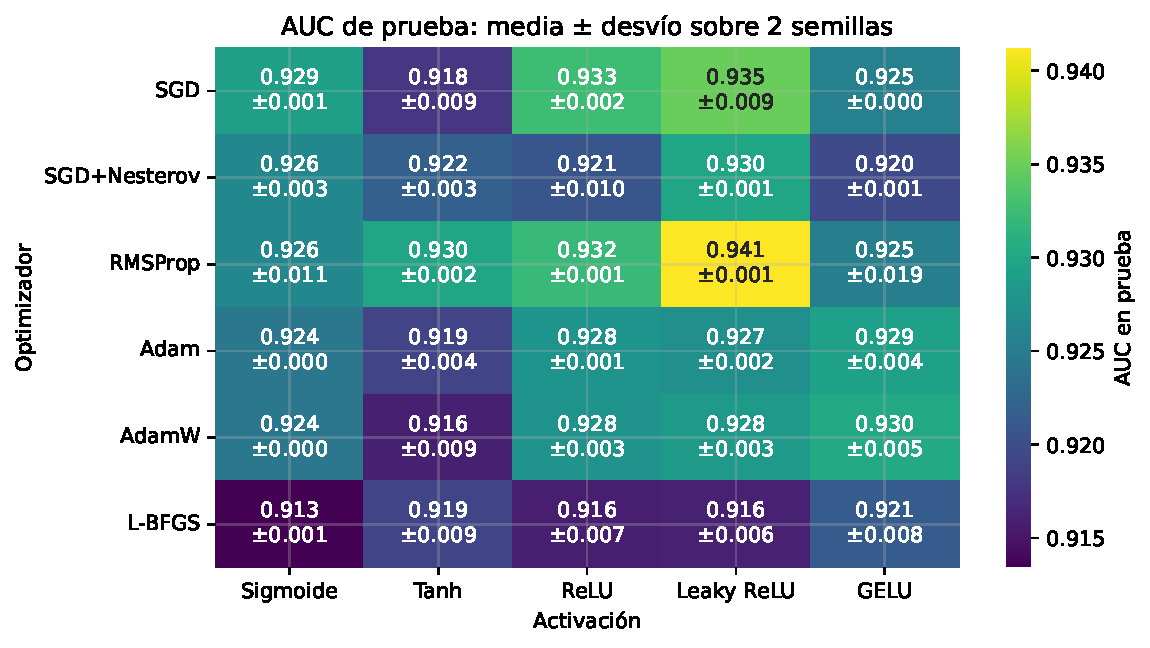
\includegraphics[width=0.8\linewidth]{grilla_heatmap_auc}
\caption{AUC de prueba (media $\pm$ desvío entre semillas) para cada combinación de optimizador y activación.}
\label{fig:heatmap}
\end{figure}

\pendiente{tasas elegidas, Friedman, rangos medios, Wilcoxon-Holm.}

\section{Funciones de activación e interacción (H2, H4)}

\begin{figure}[ht]
\centering
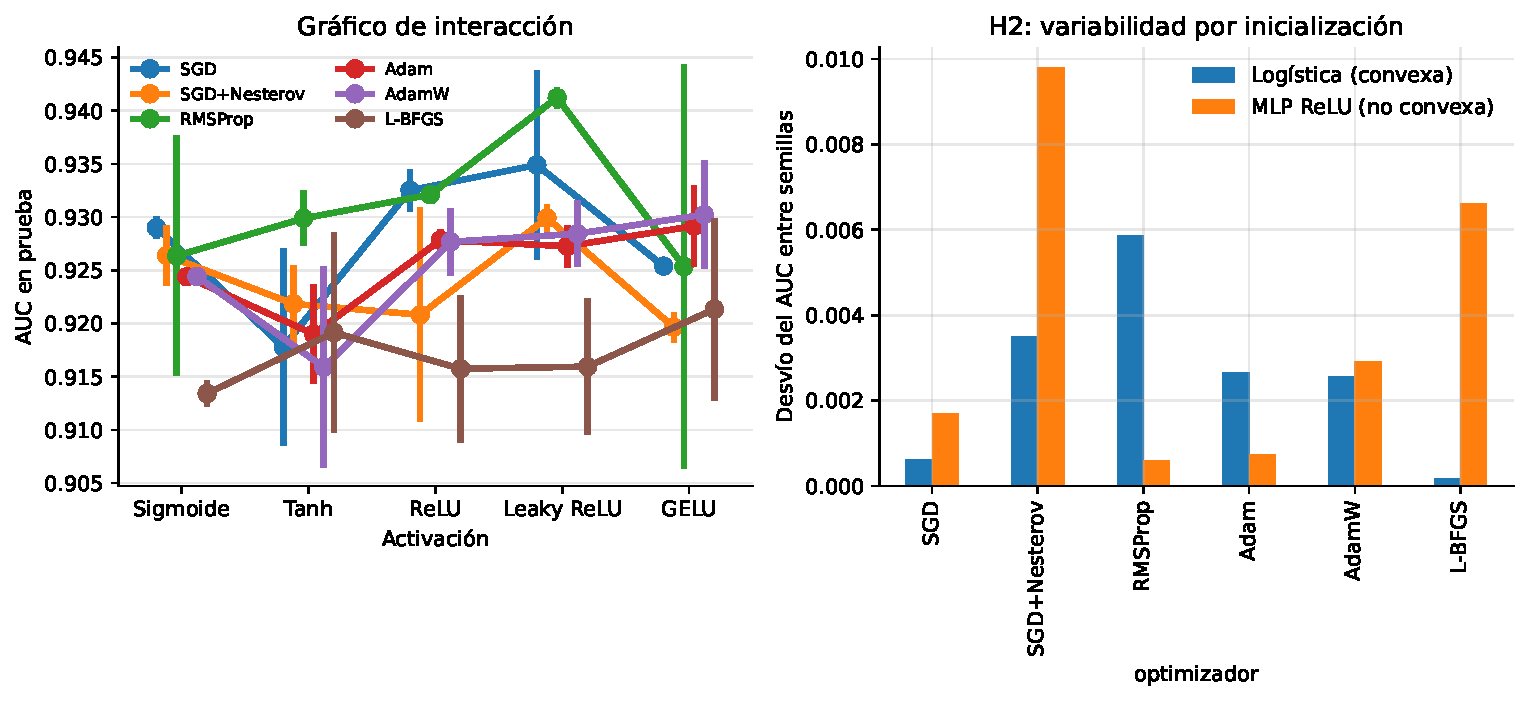
\includegraphics[width=\linewidth]{grilla_interaccion_variabilidad}
\caption{Izquierda: gráfico de interacción optimizador $\times$ activación. Derecha: desvío del AUC entre semillas en el caso convexo y no convexo.}
\label{fig:interaccion}
\end{figure}

\pendiente{ANOVA de dos factores y rango por optimizador.}

\section{Profundidad y desvanecimiento del gradiente (H3)}

\begin{figure}[ht]
\centering
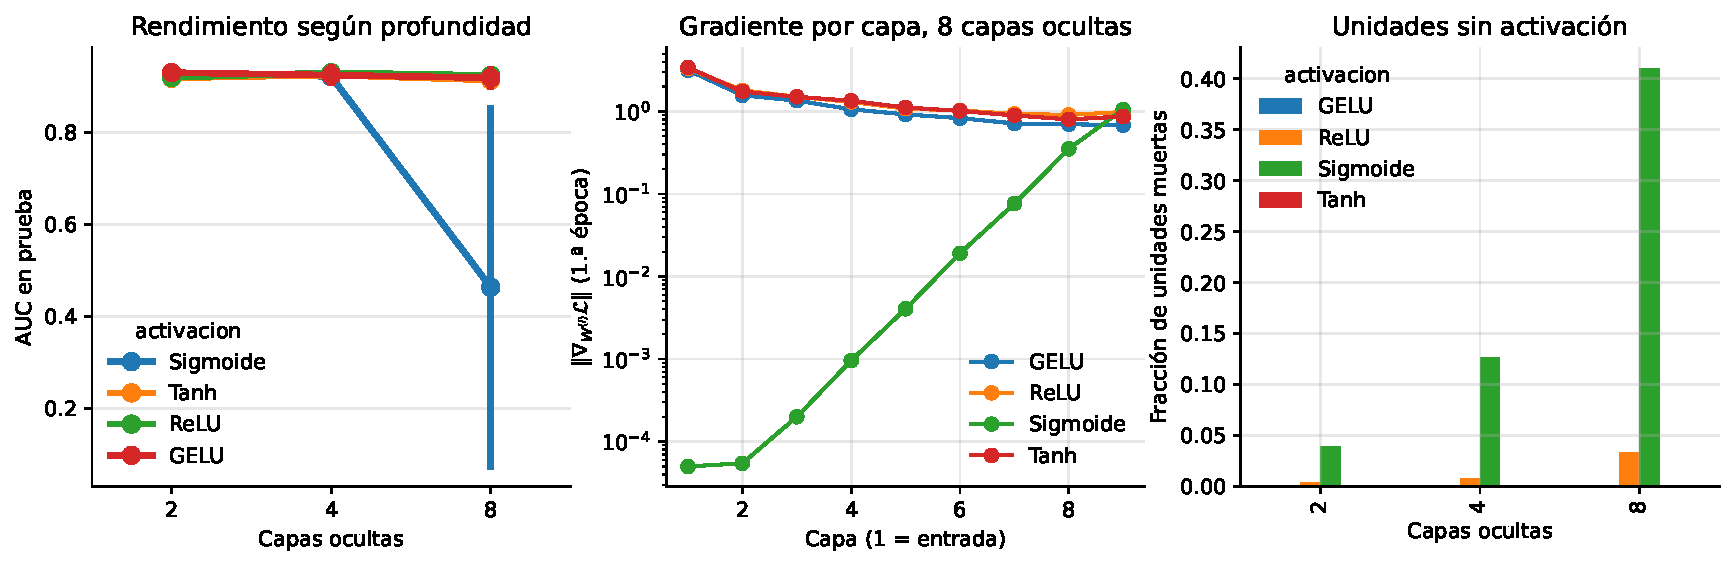
\includegraphics[width=\linewidth]{profundidad_gradientes}
\caption{AUC según profundidad, norma del gradiente por capa y fracción de unidades muertas.}
\label{fig:profundidad}
\end{figure}

\section{Evaluación del mejor modelo}

\begin{figure}[ht]
\centering
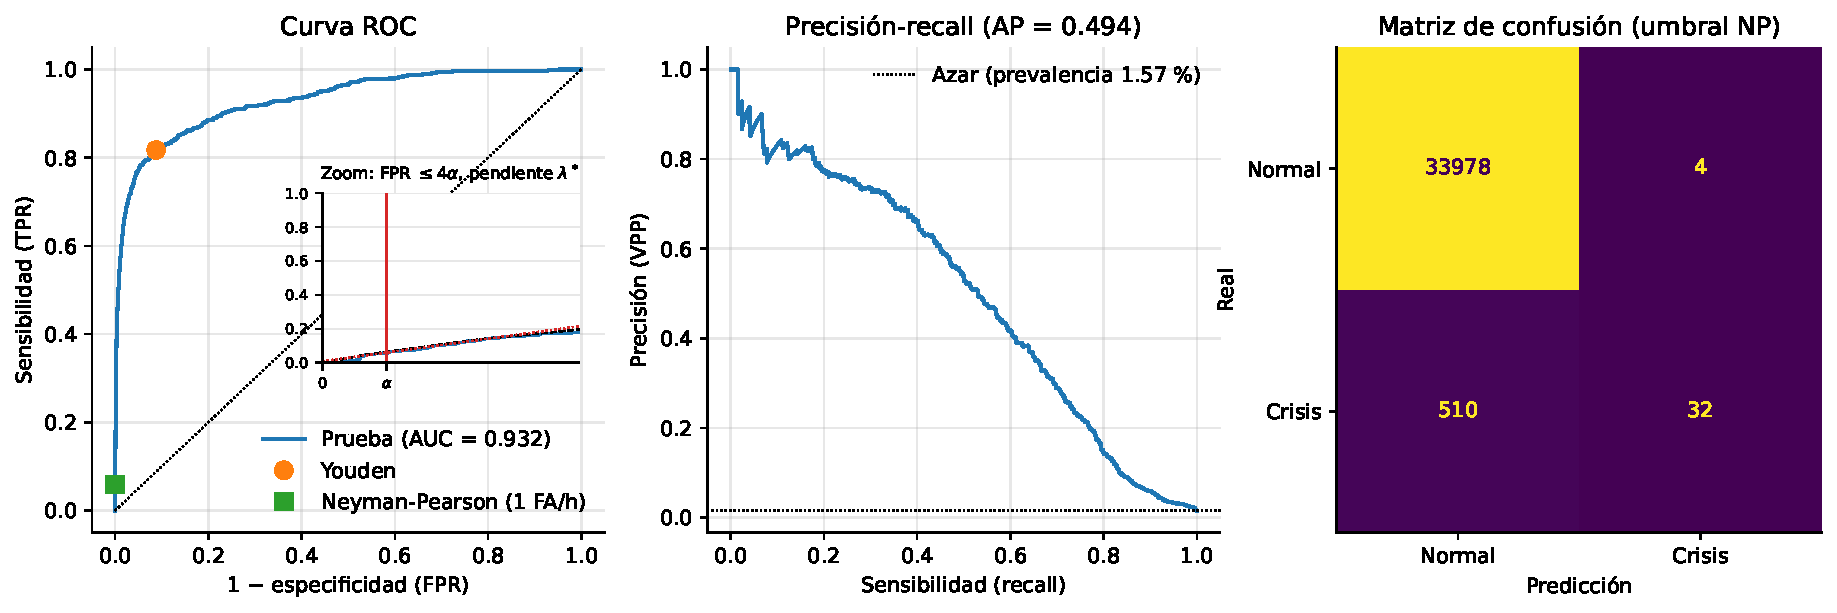
\includegraphics[width=\linewidth]{evaluacion_final}
\caption{Curva ROC (con el detalle de la región $\FPR\le 4\alpha$ y la pendiente $\lambda^\star$), curva precisión-recall y matriz de confusión con el umbral de Neyman-Pearson.}
\label{fig:evaluacion}
\end{figure}

\pendiente{tabla Youden vs. Neyman-Pearson; métricas por sujeto y por evento.}

\section{Sobreajuste}

\begin{figure}[ht]
\centering
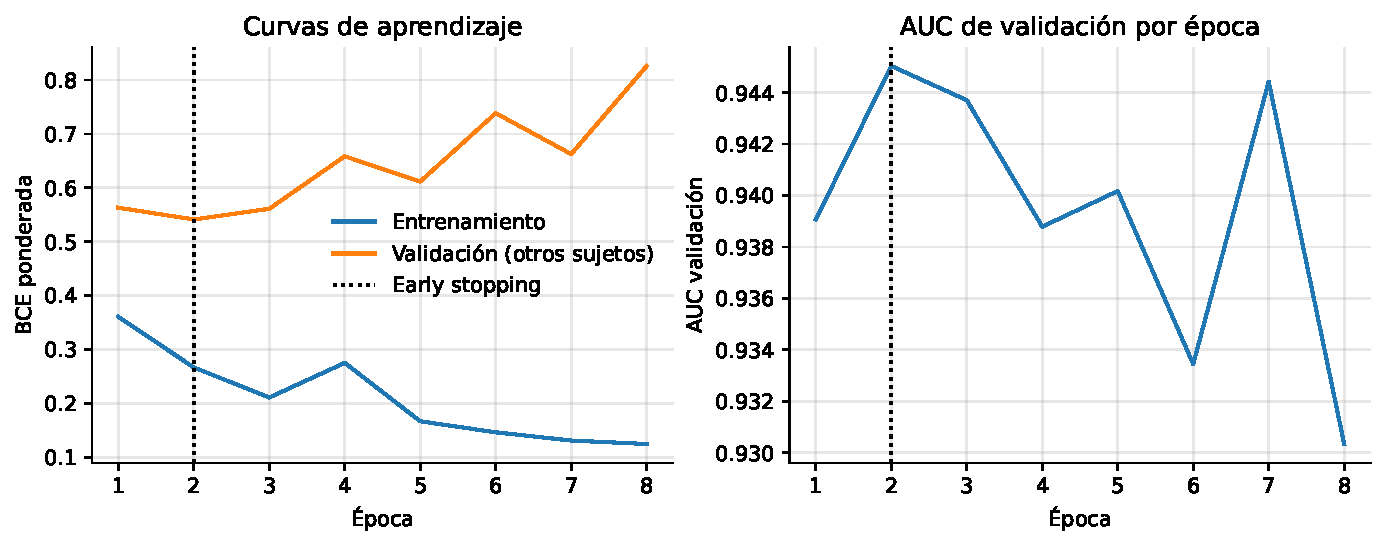
\includegraphics[width=\linewidth]{sobreajuste_curvas}
\caption{Curvas de pérdida y AUC de validación del mejor modelo.}
\label{fig:sobreajuste}
\end{figure}

\chapter{Discusión y conclusiones}
\label{cap:conclusiones}

\section{Resumen de hipótesis}
\pendiente{tabla con la evidencia de cada hipótesis (salida \texttt{resultados/resumen\_hipotesis.csv}).}

\section{Discusión}
\pendiente{interpretación de resultados; comparación con la literatura (p.~ej.\ \cite{shoeb2010}); relevancia clínica del umbral de 1 falsa alarma por hora.}

\section{Limitaciones}
\begin{itemize}
  \item Solo se usó una muestra de los registros sin crisis, lo que aumenta artificialmente la prevalencia respecto de un monitoreo continuo.
  \item La base es pediátrica y de un solo centro.
  \item El modelo clasifica ventanas independientes, sin aprovechar la continuidad temporal.
\end{itemize}

\section{Trabajo futuro}
\begin{itemize}
  \item Redes convolucionales sobre el espectrograma, tratado como imagen \parencite{gonzalez2018}.
  \item Clasificación multiclase (preictal, ictal, interictal) con salida softmax en el simplex.
  \item Suavizado temporal de las decisiones y evaluación en registros continuos completos.
\end{itemize}


\nocite{bishop2024,goodfellow2016,duda2001,buduma2022,gonzalez2018}
\printbibliography[heading=bibintoc,title={Bibliografía}]

\end{document}
